% Tipo de documento y paquetes a utilizar.
\documentclass[12pt]{article}
\usepackage[utf8]{inputenc}
% \usepackage{amsmath, amsthm, amsfonts, mathtools} % Paquete para usar más fórmulas y ecuaciones.
\usepackage{graphicx}       % Paquete para usar imágenes y figuras.
\usepackage{geometry}       % Paquete para trabajar con los márgenes del documento.
\usepackage{fancyhdr}       % Paquete para personalizar encabezado y pie de página.
\usepackage{lastpage}       % Paquete para referenciar páginas del documento.
\usepackage{listings}       % Paquete para escribir código de programación.
\usepackage{inconsolata}    % Paquete de tipo de letra consola.
\usepackage{multirow}       % Paquete para combinar filas y columnas en tablas.
\usepackage{array}          % Paquete para trabajar tablas especializadas.
\usepackage{xcolor}         % Paquete básico para agregar color al texto.
\usepackage{float}          % Paquete para utilizar fijación de figuras H.
\usepackage{hyperref}       % Paquete para insertar links en el documento.
\usepackage{comment}        % Paquete para comentarios multilínea.
\usepackage{jsstyle}        % Paquete personalizado para estilo de lstlisting para JS.

% Define colores nuevos
\definecolor{fondo_codigo}{HTML}{E4E4EE}
\definecolor{comentarios_codigo}{HTML}{3C8031}
\definecolor{enlaces}{HTML}{419CFF}

% Márgenes del documento.
\newgeometry{
    top=2.5cm,      % Superior.
    bottom=2.5cm,   % Inferior.
    outer=2.5cm,    % Parte exterior.
    inner=2.5cm,    % Parte interior.
    headheight=15pt, % Ajuste del alto del header.
    headsep=10pt,    % Ajuste del espacio entre el header y cuerpo del documento.
}

% Personalización de la cabecera y pie de página.
\pagestyle{fancy}
\fancyhf{}
\rhead{Overleaf}                                            % Texto en esquina superior derecha.
\lhead{Apuntes de Typescript}                                % Texto en esquina superior izquierda.
\rfoot{Pagina \thepage \hspace{1pt} de \pageref{LastPage}}  % Texto en esquina inferior derecha (Página n de n).
% Ancho de línea horizontal superior e inferior.
\renewcommand{\headrulewidth}{1pt}
\renewcommand{\footrulewidth}{1pt}

% Datos para la portada del documento.
\title{Apuntes de Typescript}
\author{migueluisV}
\date{Abril 2024}

% Inicio del documento.
\begin{document}

% Cambia los títulos de los índices:
% Content - Índice
% List of Figures - Índice de Figuras
% List of Tables - Índice de Tablas
\renewcommand*\contentsname{Índice}
\renewcommand{\listtablename}{Índice de Tablas}
\renewcommand{\listfigurename}{Índice de Figuras}

% Inserta la portada y los índices.
\maketitle\newpage
\tableofcontents\newpage
\listoffigures\newpage
\listoftables\newpage

\hspace{0.55cm}Este documento se hizo con \textcolor{enlaces}{\href{https://es.overleaf.com/}{\textbf{Overleaf}}} y los ejemplos fueron desarrollados y probados principalmente en el \textcolor{enlaces}{\href{https://www.typescriptlang.org/play\#code/DYUwLgBARg9joEMB2MBc06KRAvBMATgK4gDcAUKJAMYIAmISC6AzoQJZIDmuEA5AAt4CPhSoQkRALYgCaCdKizeAVjHgFweZODBeO4OsicGAM07s68okjOcQdXjbtIHFctRhIW8EADotLgAKMABPAAcQGFMgnRgASnjSIA}{Playground de Typescript}}.

La información de este documento se obtuvo de un mini curso de Youtube: \textcolor{enlaces}{\href{https://youtu.be/fUgxxhI_bvc?si=JC9jUVCaxNaDS3_4}{parte 1}} y \textcolor{enlaces}{\href{https://youtu.be/L1ZSk-vPVKI?si=Qt65wJCFzYQnFbDn}{parte 2}} y la plantilla de Lstlisting usada para Javascript fue tomada y modificada de este \textcolor{enlaces}{\href{https://github.com/xgirma/latex-javaScript/tree/master}{repositorio}} de Github.

%\sloppy La estructura HTML de los ejemplos en este documento serán omitidos, dejando únicamente lo vital para que los ejemplos funcionen y para evitar que este trabajo sea muy largo, los ejemplos CSS y Bootstrap si vendrán completos.

% Incluye los archivos que conforman al proyecto.
\section{Introducción}


\subsection{¿Qué es Typescript?}

Typescript (TS) es un súper set de Javascript (JS), es lo mismo pero con una sintaxis para tipos de datos. Se puede ver como una extensión de JS (Figura \ref{fig:1}).
\begin{figure}[H]
    \centering
    \caption{Visualización de TS sobre JS}
    \label{fig:1}
    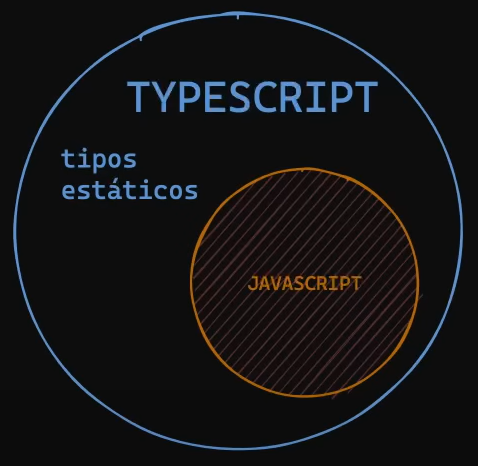
\includegraphics[width=\textwidth]{ss/1.png}
\end{figure}

TS no es un lenguaje de programación aparte como tal. TS no funciona en tiempo de ejecución, lo que llega al buscador como tal es JS. Esto es lo que el buscador recibiría de TS (\ref{tab:1}):
\begin{table}[H]
    \centering
    \caption{Código JS generado de TS}
    \label{tab:1}
    \begin{tabular}{|m{7cm}|m{7cm}|}
        \hline
        \textbf{Buscador (JS)} & \textbf{Servidor (TS)} \\
        \hline
        \parbox{7cm}{"use strict"; \\ const nombre = 'Miguel'} & const nombre = 'Miguel' \\
        \hline
    \end{tabular}
\end{table}


\subsection{¿Porqué aprenderlo?}

\begin{itemize}
    \item Por popularidad.
    \item Los tipos de datos.
    \item Mayor control sobre los resultados de funciones según los parámetros pasados.
\end{itemize}

El siguiente código muestra la clara diferencia con respecto a los tipos de datos entre TS y JS:
\begin{table}[H]
    \centering
    \caption{Aplicación de TS a código básico de JS}
    \label{tab:2}
    \begin{tabular}{|m{4cm}|m{6cm}|m{4cm}|}
        \hline
        \textbf{Lenguaje} & \textbf{Código} & \textbf{Resultado} \\
        \hline
        JS & \parbox{6cm}{function suma(a, b) \{ \\ return a + b \\ \}} & \parbox{4cm}{suma(4, 'hola') \\ '4hola'} \\
        \hline
        TS & \parbox{6cm}{function suma(a, b) \{ \\ return a + b \\ \}} & Error \\
        \hline
    \end{tabular}
\end{table}

El código de JS te permite hacer la suma de dos tipos (siempre y cuando se pueda) pero no sabes a ciencia exacta qué tipos de datos puede llegar a ingresar el usuario, haciendo vulnerable el código a cosas que no se pueden predecir. Con TS en cambio, le dices que tipo esperas en una función y qué tipo regresará, controlando los las entradas y salidas. El código de JS en TS anterior muestra un error porque no se le indica a TS el tipo de los parámetros de la función \textbf{suma}.



\section{¿Qué es la inferencia?}

La inferencia de TS se refiere a que el propio TS lee el código que estamos desarrollando e infiere (supone) el tipo de dato de las variables, funciones u objetos que estamos creando, si tenemos estos dos ejemplos:
\begin{lstlisting}
let mascota = 'mia';

const persona = {
    name = 'juan',
    age = 30
}
\end{lstlisting}

TS infiere que la variable \textit{mascota} es de tipo string por el valor contenido en esa variable, infiere que los atributos \textit{persona.name} y \textit{persona.age} son de tipo string y number, se le puede decir explícitamente el tipo, pero TS tiene esta cualidad de que infiere los tipos de las cosas. La manera de asignar un tipo a una variable, objeto o función es la siguiente 
\begin{lstlisting}
let booleano: boolean = true;
let cadena: string = 'hola';
let numero: number = 5;
let nulo: null = null;
let indefinido: undefined;
let cualquiera: any;
let desconocido: unknown;
\end{lstlisting}

Los tipos de datos básicos de JS son las cadenas (string), números (number), booleanos (boolean), null y undefined. Se utiliza el nombre de la variable, dos puntos y el tipo esperado, lo mismo para las propiedades de objetos, el valor de retorno de una función y las variables. Si se utiliza el método \textbf{typeof} con las variables tipo \textit{any} y \textit{unknown} lo que se regresará es el valor undefined.

Se recomienda ESCRIBIR LA MENOR CANTIDAD DE TIPOS DE DATOS en las variables, objetos o funciones, de eso se tiene que encargar TS. Se recomienda principalmente en variables u objetos que utilicen los tipos sencillos que se mencionaron anteriormente, para cosas más pesadas, como objetos de dependencias internas y externas, conexiones a bases de datos y otras cosas, es preferible especificar el tipo.


\subsection{Inferencia con las funciones y sus parámetros}

Por lo general, TS si logra inferir el tipo de los parámetros de una función, incluso el tipo del retorno de la función, en cualquier caso se recomienda revisar qué es lo que dice el IDE, editor de texto o TS con respecto al tipo inferido, si es any, asignar el tipo que realmente se espera, esto con el fin de seguir la regla de escribir la menor cantidad de tipos posibles.

En caso de mandar un objeto como parámetro a una función sin haberlo declarado antes también se recibe este objeto como any en todas sus propiedades, por lo que es recomendable tiparlo para evitar conflictos. Se puede tipar de dos maneras:
\begin{lstlisting}
// opcion 2
function saludar({name, age}: {name: string, age: number}) {
    console.log(`Hola ${name} y tu edad es ${age}.`);
}

// opcion 2
function saludar(persona: {name: string, age: number}) {
    const { name, age } = persona
    console.log(`Hola ${name}, y tu edad es ${age}.`);
}
\end{lstlisting}

Con la segunda manera tendríamos que hacer \textit{destructuring} del objeto para acceder a sus propiedades.


\subsection{Inferencia en funciones como parámetro}

Como sabemos, las funciones en JS se pueden usar como parámetro dentro de otra función, y el tipado tiene que ver con esta forma de trabajar los parámetros. Pongamos el siguiente ejemplo:
\begin{lstlisting}
const sayHiFromFunction = (fn) => {
    return fn('Miguel')
}

sayHiFromFunction((name) => {
    console.log(`Hola ${name}$`)
})
\end{lstlisting}

TS tendría el problema de no poder identificar el tipo del parámetro \textbf{fn} y \textbf{name}, sabe que es una función parámetro pero no sabe qué tipo es, por lo que le asignará un tipo \textbf{any}, y como se ha dicho anteriormente, debemos evitar usar este tipo lo más que se pueda.

Hay una especia de tipo llamada Function, la cual le indica a JS que una función es una función como tal de manera muy general, es como asignarle el tipo Function a una función; utilizar este tipo para tipar una función es incorrecto, ya que si, una función será un tipo función, pero para los fines de lo que regresa o no nuestra función es incorrecto, las funciones siempre se deben de tipar según el tipo que vayan a retornar (si no retornan nada, se tipan como \textbf{void})

Solucionando el ejemplo anterior, quedaría de la siguiente manera:
\begin{lstlisting}
const sayHiFromFunction = (fn: (name: string) => void) => {
    return fn('Miguel')
}

const sayHi = (name: string) => {
    console.log(`Hola ${name}$`)
}

sayHiFromFunction(sayHi)
\end{lstlisting}

La función sayHi (que antes estaba insertada dentro de los parámetros de sayHiFromFunction) no regresa nada, pero tiene un parámetro string, por lo que sayHiFromFunction se tipa como que tiene una función parámetro que a la vez tiene un parámetro (\textit{fn: (name: string)}) y no retorna nada (\textit{fn: (name: string) =$>$ void}).


\subsection{Inferencia en funciones anónimas}

Por lo general, TS si logra inferir correctamente el tipo de una función anónima, pondremos de ejemplo lo siguiente:
\begin{lstlisting}
const avengers = ['spiderman', 'hulk', 'avengers']

avengers.forEach(function (avenger) {
    console.log(avenger.toUpperCase())
})    
\end{lstlisting}

El arreglo \textbf{avengers} es de tipo string por la inferencia de TS, al usar un método de arreglos (forEach) el cual solicita una función que realice una acción, TS infiere que la función a utilizar también es string, esto por el tipo del arreglo.



\section{Asignando tipos de datos}


\subsection{Funciones regulares}

Para tipar una función regular (que utiliza la palabra reservada function), se hace de la siguiente manera:
\begin{lstlisting}
function sumar(a: number, b: number) : number {
    return a + b;
}
\end{lstlisting}


\subsection{Funciones arrow}

Para tipar una función arrow, se hace de la siguiente manera:
\begin{lstlisting}
const sumar = (a: number, b: number): number => {
    return a + b
}
\end{lstlisting}


\subsection{Funciones anónimas}

Recordemos que una función anónima es aquella que son aquellas que no han sido declaradas con un nombre, generalmente las encontramos en las funciones utilizadas por arreglos (map o filter por ejemplo). Se tipan de la siguiente manera:
\begin{lstlisting}
const arreglo = ['a', 'b', 'c']

arreglo.forEach((item: string) => {
    console.log(item)
})
\end{lstlisting}


\subsection{Tipos especiales de TS}

El tipo \textbf{any} se utiliza para, literalmente, decirle a TS que la variable u objeto puede ser de cualquier tipo, por lo cual, el lenguaje deja de recomendarnos métodos especiales para los tipos existente. Dicho en otras palabras, con any se ignora completamente el tipado que ofrece TS. Se recomienda usar lo menos posible este tipo.

El tipo \textbf{unknown} se utiliza cuando uno no sabe el tipo de dato que esperar de una variable, asignando este tipo a una variable TS no recomienda métodos especiales para tipos porque no sabe el tipo de la variable u objeto.

El tipo \textbf{never} se utiliza cuando se tiene una función donde se tiene una certeza del 100\% de que esta no devolverá ningún tipo de variable. Generalmente se utiliza en funciones que lanzan un mensaje de error como la siguiente:
\begin{lstlisting}
function throwError(message: string): never {
    throw new Error(message);
}
\end{lstlisting}

Otro ejemplo un poco más claro sobre la aparición del tipo never:
\begin{lstlisting}
function fn(x: string | number) {
    if(typeof x == 'string') {
        // type string.
        // do something.
    }
    else if(typeof x == 'number') {
        // type number.
        // do something.
    }
    else {
        x // type never.
    }
}
\end{lstlisting}



\section{Tipos propios}


\subsection{Types alias}

Podemos crear alguna especie de tipo de dato para asignárselo a objetos y que estos tengan un tipo de dato en lugar de que sean simplemente objetos sin tipo; podría decirse que es como crear una clase, la clase es una clase como tal y tiene propiedades y métodos dentro de ella que son de cierto tipo, luego podemos crear objetos de la clase y estos objetos son del tipo de la clase. Visto en C\# se ve así:
\begin{lstlisting}
// se crea la clase.
class Persona
{
    // metodos y atributos de cierto tipo.
    public string Nombre;
    public int Edad;
}

// se crea el objeto.
Persona persona = new Persona();
\end{lstlisting}

Con los type alias sería así:
\begin{lstlisting}
// se crea el alias.
type Persona = {
    Nombre: string
    Edad: number
}

let persona: Persona = {
    Nombre: 'thor',
    Edad: 1500
}
\end{lstlisting}

Ahora el objeto tiene un tipo definido.


\subsection{Union types}

Podemos crear un tipo el cual solamente pueda recibir ciertos valores o cierto tipo de dato, para el primer caso, es como si tuviéramos un if o switch donde, según el valor recibido, se le asigne otro valor a una variable, para el segundo caso, podemos decirle TS que la variable que estamos declarando puede ser un número o una cadena, una cadena o un booleano, un número o booleano, etc.

Veamos ambos casos
\begin{lstlisting}
type heroLevel = 'low' | 'medium' | 'high'

var a : number | string

var hero1 : heroLevel = 'extreme' // error.
var hero2 : heroLevel = 'low' // correcto.
a = true // error.
a = 2 // correcto.
\end{lstlisting}

Incluso se puede optar por un tipo o un valor concreto:
\begin{lstlisting}
var b : number | 'hola'
\end{lstlisting}


\subsection{Templates union types}

Podemos crear un tipo que esté constituido de otros tipos según un patrón o las necesidades que tengamos, por ejemplo, hablando de los Ids, podemos crear un formato de Id donde aparezcan 3 cadenas separadas por un guión:
\begin{lstlisting}
type PersonaId = `${string}-${string}-${string}`
\end{lstlisting}

Este tipo ahora se puede usar dentro de objetos u otros tipos:
\begin{lstlisting}
type Persona = {
    Id: PersonaId
    Nombre: string
    Edad: number
}
\end{lstlisting}


\subsection{Propiedades opcionales}

Como vimos anteriormente, podemos crear types alias, los cuales tienen propiedades de cierto tipo, podemos hacer que algunas de estas propiedades no sean obligatorias al momento de aplicar estos alias a objetos mediante el símbolo ?:
\begin{lstlisting}
type Persona = {
    Id?: PersonaId
    Nombre: string
    Edad: number
}
\end{lstlisting}

Ahora, cuando se cree un objeto tipo Persona, no será obligatorio rellenar la propiedad Id.


\subsection{Intersection types}

Otra cosa muy interesante que se puede hacer es poder combinar tipos diferentes en uno solo, armando así un nuevo tipo constituido de otros, veamos este ejemplo: tenemos un tipo HeroBasicInfo, el cual contiene dos atributos obligatorios que son el nombre y edad de un héroe, también tenemos HeroProperties, el cual tiene otros atributos no obligatorios del héroe, como sería su status y escala de poder:

\begin{lstlisting}
type heroLevel = 'low' | 'medium' | 'high'

type HeroBasicInfo = {
    nombre: string,
    edad: number
}

type HeroProperties = {
    isActive?: boolean,
    powerScale?: heroLevel
}
\end{lstlisting}

HeroLevel es un complemento visto en uno de los ejemplos anteriores. Si queremos combinar estos dos tipos se hace de la siguiente manera:
\begin{lstlisting}
type Hero = HeroBasicInfo & HeroProperties;

let hero3 = {
    name: 'spiderman',
    age: 30
}
\end{lstlisting}

De esta manera, tenemos los atributos de ambos tipos en uno solo, así el tipo puede recibir menor cantidad de atributos y aligerar la carga de trabajo.


\subsection{Types indexing}

En caso de que tengamos un tipo con un objeto como atributo, al momento de querer acceder a este objeto y querer asignar valores en una variable o constante, podemos utilizar el type indexing para lograr este cometido:
\begin{lstlisting}
type HeroProperties = {
    isActive: boolean,
    address: {
        planet: string,
        city: string
    }
}

const addressHero: HeroProperties['address'] = {
    planet: 'Tierra',
    city: 'Madrid'
}
\end{lstlisting}

Vemos que se crea el tipo HeroProperties el cual tiene un objeto llamado 'address' dentro, al crear una variable tipo HeroProperties, podemos acceder al objeto dentro del tipo solamente utilizando los corchetes con el nombre del objeto que deseamos utilizar, como se ve en la constante addressHero.


\subsection{Types de valores y funciones}

Si declaramos un objeto con ciertos atributos de x tipo, podemos crear un tipo que sea igual a este objeto:
\begin{lstlisting}
const address = {
    planet: 'Tierra',
    city: 'Madrid'
}

type Address = typeof address
\end{lstlisting}

Esto se puede transportar a lo que regresa un función:
\begin{lstlisting}
function createAddress() {
    return {
        planet: 'Tierra',
        city: 'Madrid'
    }
}

type Address = ReturnType<typeof createAddress>
\end{lstlisting}

ReturnType recupera el tipo de alguna función que le pases, en este caso recupera el tipo del objeto que regresa la función createAddress, el cual es un objeto con dos atributos tipo string.

\section{Colecciones de datos}


\subsection{Arreglos}

La forma típica para declarar un arreglo en JS es la siguiente:
\begin{lstlisting}
const languages = [];
\end{lstlisting}

Sin embargo, TS tendrá problemas al hacer esto, ya que esta forma de declaración le está diciendo a TS que este arreglo siempre contendrá valores tipo \textit{never} (visto en los tipos especiales de TS), por lo que, si intentamos hacer un push con cualquier tipo de valor, tendremos problemas.

La manera correcta de declarar un arreglo en TS es remarcando el tipo de dato del arreglo:
\begin{lstlisting}
// opcion 1.
const languages: string[] = []

// opcion 2.
const languages: Array<string> = []
\end{lstlisting}

¿Cuál de las dos escoger?, depende de los gustos.

¿Qué pasa si quiere almacenar dos o más tipos en mi arreglo?, esta es la manera correcta e incorrecta de hacerlo:
\begin{lstlisting}
// incorrecto.
const languages: Arrary<string> | Array<number> = []
const languages: string[] | number[] = []

// correcto.
const languages: (string | number)[] = []
\end{lstlisting}

\textit{Nota:} utilizando el Playground de TS, la forma \textit{const languages: Arrary$<$string$>$ $|$ Array$<$number$>$ = []} parece ser que también es correcta.


\subsection{Matrices y Tuplas}

Una matriz es una colección de datos de n dimensiones mayores a lo que vendría siendo un arreglo convencional, una tupla es una colección de datos que se puede encontrar en diferentes lenguajes de programación, suele ser una agrupación de datos que, por su naturaleza, vienen todos juntos, esta agrupación suele ser de un mismo número de valores y tipo.

Las tuplas y matrices también pueden ser creadas en TS según el tipo de declaración de TS, veamos el siguiente ejemplo: tenemos el juego del gato, donde tenemos una matriz 3x3 y ponemos los típicos valores 'x' ó 'o', tendría este aspecto:
\begin{lstlisting}
['x', 'o', 'o']
['o', 'x', 'o']
['o', 'o', 'x']
\end{lstlisting}

Para lograr esto, lo primero que se nos podría ocurrir sería crear un arreglo de arreglos:
\begin{lstlisting}
const gameBoard: string[][] = {
    ['x', 'o', 'o'],
    ['o', 'x', 'o'],
    ['o', 'o', 'x']
}
\end{lstlisting}

El gran detalle con esto es que podemos seguir asignando valores a este arreglo de arreglos y podemos asignarle algo diferente a los valores esperados (asignar el valor '234effdf3e' en lugar de 'x' o 'o'). Si hacemos la corrección queda así:
\begin{lstlisting}
type Cells = 'x' | 'o' | ''
type GameBoard = [
    [Cells, Cells, Cells],
    [Cells, Cells, Cells],
    [Cells, Cells, Cells]
]

const gameBoard: GameBoard = [
    ['x', 'o', 'o'],
    ['o', 'x', 'o'],
    ['o', 'o', 'x']
]
\end{lstlisting}

Con esto, primero definimos el tipo donde se aceptan solo los valores que deseamos (\textit{Cells}), luego definimos otro tipo que solo contenga arreglos de tres elementos tipo Cells (\textit{GameBoard}), finalmente declaramos una constante que es del tipo GameBoard y con eso satisface todas las necesidades correspondientes a una matriz 3x3 con los valores requeridos solamente.

Un problema con las tuplas es que son mutables (error del lenguaje directamente), si utilizamos el siguiente código:
\begin{lstlisting}
type RGB = [number, number, number]

const rgb: RGB = [0,0,0]

rgb.push(4)
\end{lstlisting}

Ahora la constante \textit{rgb} tendrá cuatro espacios o variables para almacenar datos, este error es del lenguaje y no ha habido solución, por lo que, si no quieres que se acceda a la información de la tupla, la puedes volver \textit{readonly}:
\begin{lstlisting}
type RGB = readonly [number, number, number]
\end{lstlisting}


\subsection{Enums}

Los \textit{enums} son un tipo de colección de datos donde se almacena una lista de valores conocidos, esta lista es finita y suele ser corta, de alrededor de 20 itemos por enum.

Los enums no existen en JS, por lo que al momento de utilizarlos en TS toman otro aspecto que veremos más adelante, por lo pronto, esta es la sintaxis para declarar un enum:
\begin{lstlisting}
enum ERROR_TYPES {
    NOT_FOUND,
    UNAUTHORIZED,
    FORBIDDEN
}

function mostrarMensaje(tipoDeError: ERROR_TYPES) {
    if(tipoDeError == ERROR_TYPES.NOT_FOUND)
        console.log('No se encuentra el recurso')
    else if(tipoDeError == ERROR_TYPES.UNAUTHORIZ)
        console.log('No tienes el permiso para acceder')
    else if(tipoDeError == ERROR_TYPES.FORBIDDEN)
        console.log('Error')
}
\end{lstlisting}

Vemos que se suelen utilizar con listas de cosas que ya conocemos, como una lista de tipos de errores, sexos, días de la semana, meses, etc. Se declara el enum con sus valores y se puede utilizar en código. Recordemos que los enums no existen en JS, por lo que si vemos en el compilador online de TS:
\begin{lstlisting}
"use strict";
var ERROR_TYPES;
(function (ERROR_TYPES) {
    ERROR_TYPES[ERROR_TYPES["NOT_FOUND"] = 0] = "NOT_FOUND";
    ERROR_TYPES[ERROR_TYPES["UNAUTHORIZED"] = 1] = "UNAUTHORIZED";
    ERROR_TYPES[ERROR_TYPES["FORBIDDEN"] = 2] = "FORBIDDEN";
})(ERROR_TYPES || (ERROR_TYPES = {}));
function mostrarMensaje(tipoDeError) {
    if (tipoDeError == ERROR_TYPES.NOT_FOUND)
        console.log('No se encuentra el recurso');
    else if (tipoDeError == ERROR_TYPES.UNAUTHORIZED)
        console.log('No tienes el permiso para acceder');
    else if (tipoDeError == ERROR_TYPES.FORBIDDEN)
        console.log('Error');
}
\end{lstlisting}

Esto genera muchísimo código extra, que en general declara un objeto o función que sirve para realizar la funcionalidad del enum en JS. Es mucho código, si agregamos la palabra reservada \textit{const} al inicio de nuestro enum pasa otra cosa:
\begin{lstlisting}
"use strict";
function mostrarMensaje(tipoDeError) {
    if (tipoDeError == 0 /* ERROR_TYPES.NOT_FOUND */)
        console.log('No se encuentra el recurso');
    else if (tipoDeError == 1 /* ERROR_TYPES.UNAUTHORIZED */)
        console.log('No tienes el permiso para acceder');
    else if (tipoDeError == 2 /* ERROR_TYPES.FORBIDDEN */)
        console.log('Error');
}
\end{lstlisting}

Nos hemos desecho del código extra y se sustituye el rastro del enum con unos valores numéricos \textbf{comenzando desde el 0} (para este caso del \textit{if}). Pero aquí podrás pensar que tal vez no quieras utilizar estos índices, que prefieres utilizar cadenas de texto, hay una solución para eso:

\textbf{Código TS}
\begin{lstlisting}
const enum ERROR_TYPES {
    NOT_FOUND = 'not found',
    UNAUTHORIZED = 'unauthorized',
    FORBIDDEN = 'forbidden'
}

function mostrarMensaje(tipoDeError: ERROR_TYPES) {
    if(tipoDeError == ERROR_TYPES.NOT_FOUND)
        console.log('No se encuentra el recurso')
    else if(tipoDeError == ERROR_TYPES.UNAUTHORIZED)
        console.log('No tienes el permiso para acceder')
    else if(tipoDeError == ERROR_TYPES.FORBIDDEN)
        console.log('Error')
}
\end{lstlisting}

\textbf{Código JS compilado}
\begin{lstlisting}
"use strict";
function mostrarMensaje(tipoDeError) {
    /* ERROR_TYPES.NOT_FOUND */
    if (tipoDeError == "not found")
        console.log('No se encuentra el recurso');
    /* ERROR_TYPES.UNAUTHORIZED */
    else if (tipoDeError == "unauthorized")
        console.log('No tienes el permiso para acceder');
    /* ERROR_TYPES.FORBIDDEN */
    else if (tipoDeError == "forbidden")
        console.log('Error');
}
\end{lstlisting}

Se sustituyen los valores numéricos por cadenas de texto, si quitamos el \textit{const} en este segundo caso no habría inconveniente alguno.

\textbf{¿Cuál utilizar?, ¿Con o sin \textit{const}?}

Esta pregunta se responde viendo para qué es el proyecto, si tu proyecto es interno y no habrá un tercero que lo consumirá como un servicio o librería, puedes utilizar los enums con \textit{const}, si fuera caso contrario se recomienda omitir este último para que, quien te consuma, vea el código generado del enum.



\section{Aserciones}


\subsection{Con elementos HTML}

Recordemos que JS se utiliza en conjunto con HTML para desarrollo web, TS no se queda atrás y podemos utilizar la inferencia con los elementos HTML de nuestro proyecto, pero hay que saber utilizarlo para que el código TS funcione correctamente con el de JS (compilado y en ejecución). Tenemos el siguiente ejemplo muy sencillo
\begin{lstlisting}
const canvas = document.getElementById('canvas')

const ctx = canvas.getContext('2d')
\end{lstlisting}

Podemos recuperar los atributos e información de un elemento HTML mediante el objeto y función \textit{document.getElementById('canvas')}, algo que se ha visto en JS también, con TS podemos inferir que la constante \textit{const} es de tipo canvas o tipo HTML, existe un tipo genérico para los elementos HTML llamado \textbf{HTMLElement}, la desventaja de este tipo es que es general, no especifica qué tipo de elemento es el que queremos recuperar, para nuestra fortuna, existen tipos más específicos para nuestros elementos:
\begin{lstlisting}
const canvas = document.getElementById('canvas')
    as HTMLCanvasEelement

const ctx = canvas.getContext('2d')
\end{lstlisting}

Con esto TS ya sabe que la constante \textit{canvas} es un elemento Canvas de HTML, sin embargo, esta constante puede recibir un valor cualquiera o puede recibir \textit{null}, ya que el código no sabe si realmente recibirá un objeto canvas o no, por lo que tenemos que meter alguna condicional para asegurar que recibiremos un valor:
\begin{lstlisting}
const canvas = document.getElementById('canvas')
    as HTMLCanvasElement

if (canvas != null) {
    const ctx = canvas.getContext('2d')
}
\end{lstlisting}

El código anterior nos está atando ahora a que lo que recibamos es un elemento Canvas, pero qué pasa si recibimos algún elemento diferente (p, span, img, etc.), debemos poder asegurar también que el elemento recibido es el esperado:
\begin{lstlisting}
const canvas = document.getElementById('canvas')

if (canvas != null && canvas instanceof HTMLCanvasElement) {
    const ctx = canvas.getContext('2d')
}
\end{lstlisting}

Esta seria la solución definitiva a nivel TS y JS para nuestro problema, veamos qué aspecto tiene en código JS:
\begin{lstlisting}
"use strict";

const canvas = document.getElementById('canvas');

if (canvas != null && canvas instanceof HTMLCanvasElement) {
    const ctx = canvas.getContext('2d');
}
\end{lstlisting}

Como se puede apreciar, el código es igual en TS y en JS, la diferencia está en que TS logra inferir el tipo de elemento recibido en la constante canvas y se puede trabajar de manera más segura. ¿Qué aspecto tendría el código JS si si hubiéramos utilizado el penúltimo código TS?
\begin{lstlisting}
"use strict";

const canvas = document.getElementById('canvas');

if (canvas != null) {
    const ctx = canvas.getContext('2d');
}
\end{lstlisting}

Vemos que la instrucción \textit{as HTMLCanvasElement} al final de nuestra constante desaparece, por lo que en el futuro podríamos romper el código.


\subsection{Con Fetching}

Otra de las cosas que se suele hacer con JS es el consumir datos de una API, sabemos que se debe declarar una constante con la URL de la API que queremos que consumir y utilizar algún método para consumirla, al obtener una respuesta no negativa tenemos acceso al objeto de respuesta y con hacer lo que se requiera, con TS también podemos realizar una aserción para controlar el los datos y tipos de la respuesta de la API. Tenemos el siguiente código:
\begin{lstlisting}
const API_URL =
    "https://api.github.com/search/repositories?q=javascript"

// response es del tipo 'Response'
const response = await fetch(API_URL)

if (!response.ok) {
    throw new Error('Request failed')
}

// data es del tipo 'any', se debe indicar que tipo es.
const data = await response.json()

const repos = data.items.map(repo => {
    console.log(repo)
})
\end{lstlisting}

Como tal, TS no tiene un tipo específico para las respuestas de una API, tendríamos que crear nosotros un tipo con todos los tipos de los atributos del objeto JSON que nos retorne la respuesta de la API y asignárselo a la constante o variable.

Crear el tipo manualmente puede ser muy tardado y tedioso, existe el sitio web \textcolor{enlaces}{\href{https://app.quicktype.io/}{quicktype}} que recibe un objeto JSON como respuesta de una API y te genera el tipo personalizado con todos los tipos de los atributos del objeto, es un método más rápido para trabajar esta parte. Si acedemos a la URL de la api del código de arriba, nos regresará un JSON bastante extenso, lo copiamos y pegamos en \textit{quicktype} y nos generará los tipos automáticamente. Tome en cuenta lo siguiente:
\begin{figure}[H]
    \centering
    \caption{Área de trabajo de \textit{quicktype}}
    \label{fig:2}
    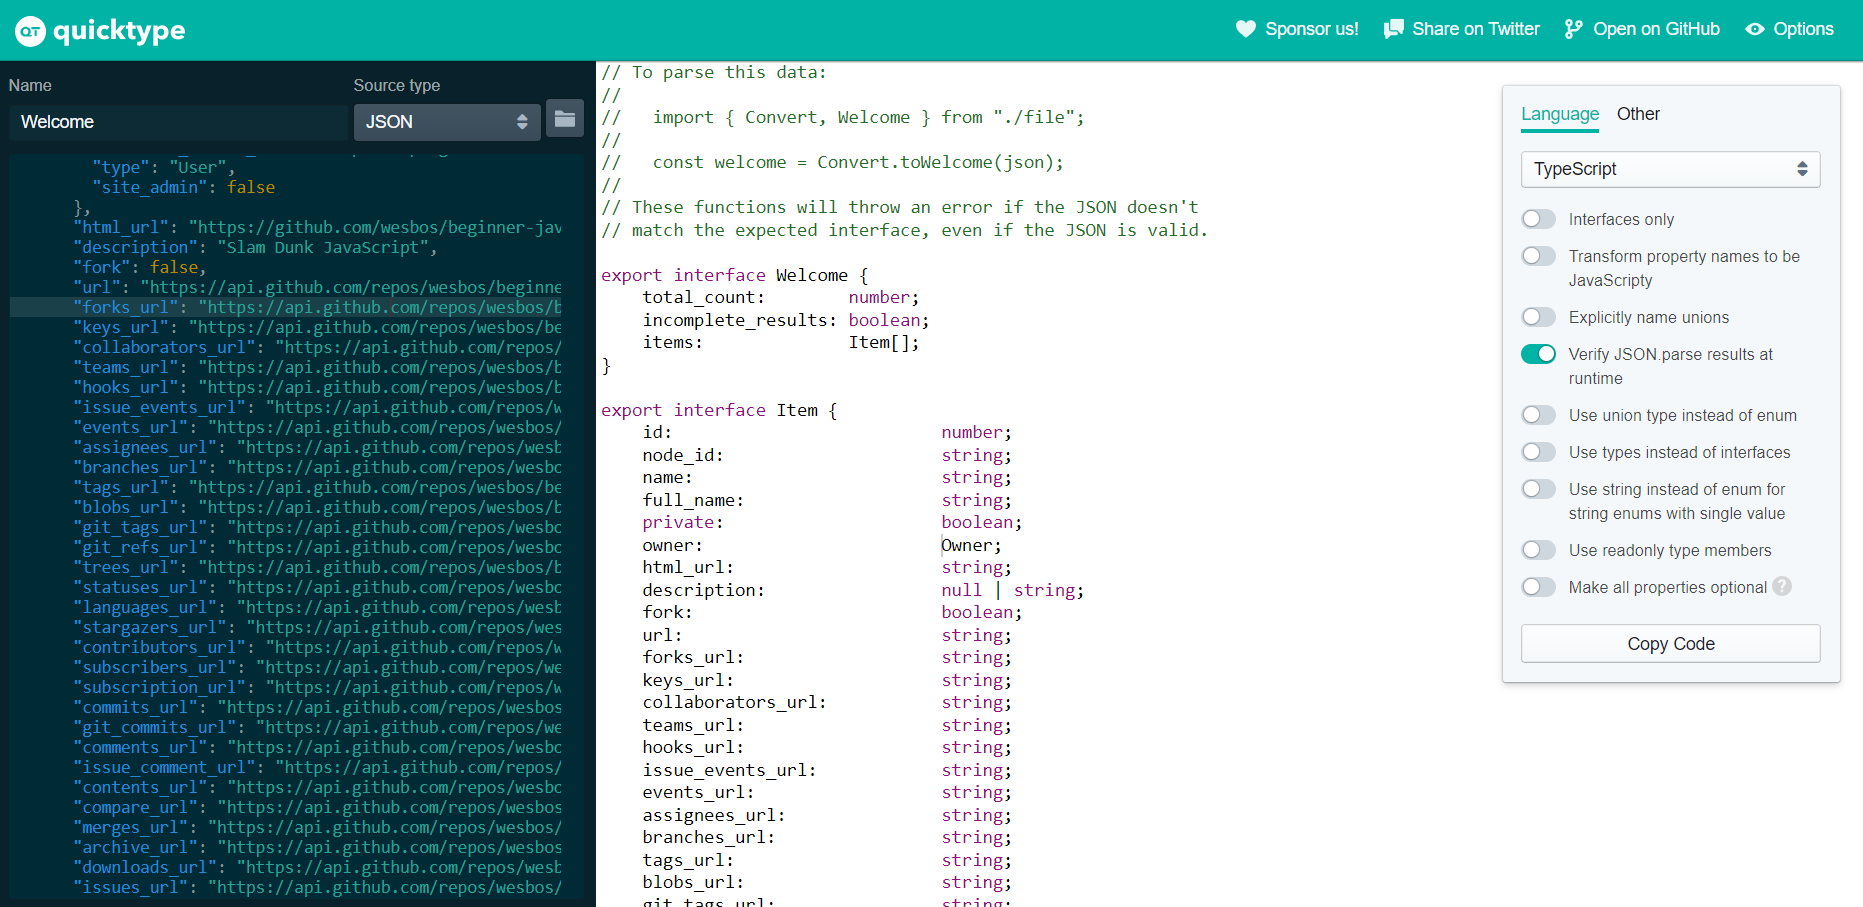
\includegraphics[width=\textwidth]{ss/2.png}
\end{figure}

\textit{Nota}: no olvidar cambiar el nombre del tipo que se va a generar en quicktype en la parte superior de la sección izquierda donde se pega la respuesta.

La figura anterior muestra el área de trabajo, vemos que en el lado derecho hay una ventana flotante con varias opciones, el lenguaje seleccionado es TS pero se pueden seleccionar más, podemos marcar y desmarcar otras opciones según nuestros requerimientos. Hay otras versiones que podemos seleccionar de TS, en especial TypeScript Zod, donde se incluye una librería para validación de tipos de datos, esta librería debe instalarse y tomará un poco más de tiempo que termine su ejecución, pero añade el factor de validación a nivel TS y JS.
\begin{figure}[H]
    \centering
    \caption{Selección del lenguaje a TypeScript Zod}
    \label{fig:3}
    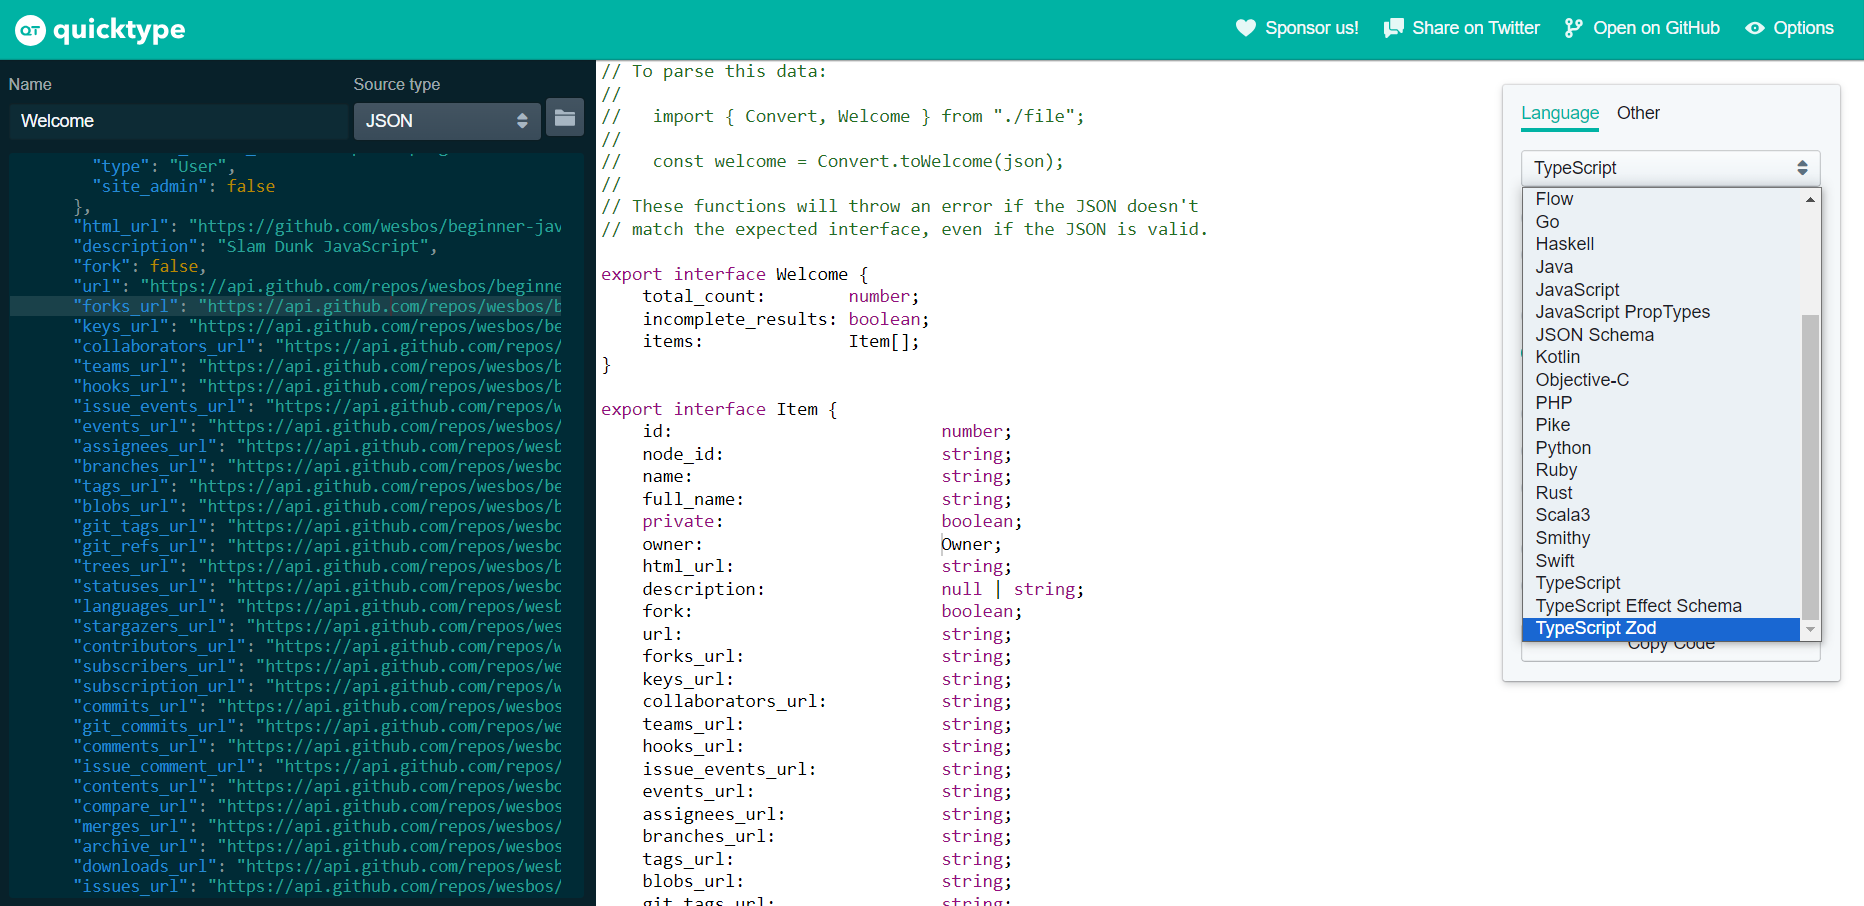
\includegraphics[width=\textwidth]{ss/3.png}
\end{figure}

Si pegamos el código generado con el lenguaje TS sin Zod en el Playground de TS, tenemos un código JS como este:
\begin{lstlisting}
// To parse this data:
//
//   import { Convert, Welcome } from "./file";
//
//   const welcome = Convert.toWelcome(json);
//
// These functions will throw an error if the JSON doesn't
// match the expected interface, even if the JSON is valid.
export var DefaultBranch;
(function (DefaultBranch) {
    DefaultBranch["Dev"] = "dev";
    DefaultBranch["Main"] = "main";
    DefaultBranch["Master"] = "master";
})(DefaultBranch || (DefaultBranch = {}));
export var Language;
(function (Language) {
    Language["CSS"] = "CSS";
    Language["HTML"] = "HTML";
    Language["JavaScript"] = "JavaScript";
    Language["TypeScript"] = "TypeScript";
})(Language || (Language = {}));
export var Type;
(function (Type) {
    Type["Organization"] = "Organization";
    Type["User"] = "User";
})(Type || (Type = {}));
export var Visibility;
(function (Visibility) {
    Visibility["Public"] = "public";
})(Visibility || (Visibility = {}));
// Converts JSON strings to/from your types
// and asserts the results of JSON.parse at runtime
export class Convert {
    static toWelcome(json) {
        return cast(JSON.parse(json), r("Welcome"));
    }
    static welcomeToJson(value) {
        return JSON.stringify
            (uncast(value, r("Welcome")), null, 2);
    }
}
function invalidValue(typ, val, key, parent = '') {
    const prettyTyp = prettyTypeName(typ);
    const parentText = parent ? ` on ${parent}` : '';
    const keyText = key ? ` for key "${key}"` : '';
    throw Error(`Invalid value${keyText}${parentText}.
        Expected ${prettyTyp} but got ${JSON.stringify(val)}`);
}
function prettyTypeName(typ) {
    if (Array.isArray(typ)) {
        if (typ.length === 2 && typ[0] === undefined) {
            return `an optional ${prettyTypeName(typ[1])}`;
        }
        else {
            return `one of [${typ.map(a =>
            {
                return prettyTypeName(a);
            }).join(", ")}]`;
        }
    }
    else if (typeof typ === "object" &&
            typ.literal !== undefined) {
        return typ.literal;
    }
    else {
        return typeof typ;
    }
}
function jsonToJSProps(typ) {
    if (typ.jsonToJS === undefined) {
        const map = {};
        typ.props.forEach((p) => map[p.json] = {
            key: p.js, typ: p.typ
        });
        typ.jsonToJS = map;
    }
    return typ.jsonToJS;
}
function jsToJSONProps(typ) {
    if (typ.jsToJSON === undefined) {
        const map = {};
        typ.props.forEach((p) => map[p.js] = {
            key: p.json, typ: p.typ
        });
        typ.jsToJSON = map;
    }
    return typ.jsToJSON;
}
function transform(val, typ, getProps, key = '', parent = '') {
    function transformPrimitive(typ, val) {
        if (typeof typ === typeof val)
            return val;
        return invalidValue(typ, val, key, parent);
    }
    function transformUnion(typs, val) {
        // val must validate against one typ in typs
        const l = typs.length;
        for (let i = 0; i < l; i++) {
            const typ = typs[i];
            try {
                return transform(val, typ, getProps);
            }
            catch (_) { }
        }
        return invalidValue(typs, val, key, parent);
    }
    function transformEnum(cases, val) {
        if (cases.indexOf(val) !== -1)
            return val;
        return invalidValue(cases.map(a => {
            return l(a);
        }), val, key, parent);
    }
    function transformArray(typ, val) {
        // val must be an array with no invalid elements
        if (!Array.isArray(val))
            return invalidValue(l("array"), val, key, parent);
        return val.map(el => transform(el, typ, getProps));
    }
    function transformDate(val) {
        if (val === null) {
            return null;
        }
        const d = new Date(val);
        if (isNaN(d.valueOf())) {
            return invalidValue(l("Date"), val, key, parent);
        }
        return d;
    }
    function transformObject(props, additional, val) {
        if (val === null ||
            typeof val !== "object" ||
            Array.isArray(val)) {
            return invalidValue
                (l(ref || "object"), val, key, parent);
        }
        const result = {};
        Object.getOwnPropertyNames(props).forEach(key => {
            const prop = props[key];
            const v = Object.prototype.hasOwnProperty
            .call(val, key)? val[key] : undefined;
            result[prop.key] = transform(v, prop.typ,
            getProps, key, ref);
        });
        Object.getOwnPropertyNames(val).forEach(key => {
            if (!Object.prototype.hasOwnProperty
            .call(props, key)) {
                result[key] = transform(val[key], additional,
                getProps, key, ref);
            }
        });
        return result;
    }
    if (typ === "any")
        return val;
    if (typ === null) {
        if (val === null)
            return val;
        return invalidValue(typ, val, key, parent);
    }
    if (typ === false)
        return invalidValue(typ, val, key, parent);
    let ref = undefined;
    while (typeof typ === "object" && typ.ref !== undefined) {
        ref = typ.ref;
        typ = typeMap[typ.ref];
    }
    if (Array.isArray(typ))
        return transformEnum(typ, val);
    if (typeof typ === "object") {
        return typ.hasOwnProperty("unionMembers") ?
        transformUnion(typ.unionMembers, val)
        :
        typ.hasOwnProperty("arrayItems") ? transformArray
            (typ.arrayItems, val)
        : 
        yp.hasOwnProperty("props") ? transformObject
            (getProps(typ), typ.additional, val)
        :
        invalidValue(typ, val, key, parent);
    }
    // Numbers can be parsed by Date but shouldn't be.
    if (typ === Date && typeof val !== "number")
        return transformDate(val);
    return transformPrimitive(typ, val);
}
function cast(val, typ) {
    return transform(val, typ, jsonToJSProps);
}
function uncast(val, typ) {
    return transform(val, typ, jsToJSONProps);
}
function l(typ) {
    return { literal: typ };
}
function a(typ) {
    return { arrayItems: typ };
}
function u(...typs) {
    return { unionMembers: typs };
}
function o(props, additional) {
    return { props, additional };
}
function m(additional) {
    return { props: [], additional };
}
function r(name) {
    return { ref: name };
}
const typeMap = {
    "Welcome": o([
        { json: "total_count", js: "total_count", typ: 0 },
        { json: "incomplete_results", js: "incomplete_results",
            typ: true },
        { json: "items", js: "items", typ: a(r("Item")) },
    ], false),
    "Item": o([
        { json: "id", js: "id", typ: 0 },
        { json: "node_id", js: "node_id", typ: "" },
        { json: "name", js: "name", typ: "" },
        { json: "full_name", js: "full_name", typ: "" },
        { json: "private", js: "private", typ: true },
        { json: "owner", js: "owner", typ: r("Owner") },
        { json: "html_url", js: "html_url", typ: "" },
        { json: "description", js: "description",
            typ: u(null, "") },
        { json: "fork", js: "fork", typ: true },
        { json: "url", js: "url", typ: "" },
        { json: "forks_url", js: "forks_url", typ: "" },
        { json: "keys_url", js: "keys_url", typ: "" },
        { json: "collaborators_url", js: "collaborators_url",
            typ: "" },
        { json: "teams_url", js: "teams_url", typ: "" },
        { json: "hooks_url", js: "hooks_url", typ: "" },
        { json: "issue_events_url", js: "issue_events_url",
            typ: "" },
        { json: "events_url", js: "events_url", typ: "" },
        { json: "assignees_url", js: "assignees_url", typ: "" },
        { json: "branches_url", js: "branches_url", typ: "" },
        { json: "tags_url", js: "tags_url", typ: "" },
        { json: "blobs_url", js: "blobs_url", typ: "" },
        { json: "git_tags_url", js: "git_tags_url", typ: "" },
        { json: "git_refs_url", js: "git_refs_url", typ: "" },
        { json: "trees_url", js: "trees_url", typ: "" },
        { json: "statuses_url", js: "statuses_url", typ: "" },
        { json: "languages_url", js: "languages_url", typ: "" },
        { json: "stargazers_url", js: "stargazers_url", typ: "" },
        { json: "contributors_url", js: "contributors_url",
            typ: "" },
        { json: "subscribers_url", js: "subscribers_url",
            typ: "" },
        { json: "subscription_url", js: "subscription_url",
            typ: "" },
        { json: "commits_url", js: "commits_url", typ: "" },
        { json: "git_commits_url", js: "git_commits_url",
            typ: "" },
        { json: "comments_url", js: "comments_url", typ: "" },
        { json: "issue_comment_url", js: "issue_comment_url",
            typ: "" },
        { json: "contents_url", js: "contents_url", typ: "" },
        { json: "compare_url", js: "compare_url", typ: "" },
        { json: "merges_url", js: "merges_url", typ: "" },
        { json: "archive_url", js: "archive_url", typ: "" },
        { json: "downloads_url", js: "downloads_url", typ: "" },
        { json: "issues_url", js: "issues_url", typ: "" },
        { json: "pulls_url", js: "pulls_url", typ: "" },
        { json: "milestones_url", js: "milestones_url", typ: "" },
        { json: "notifications_url", js: "notifications_url",
            typ: "" },
        { json: "labels_url", js: "labels_url", typ: "" },
        { json: "releases_url", js: "releases_url", typ: "" },
        { json: "deployments_url", js: "deployments_url",
            typ: "" },
        { json: "created_at", js: "created_at", typ: Date },
        { json: "updated_at", js: "updated_at", typ: Date },
        { json: "pushed_at", js: "pushed_at", typ: Date },
        { json: "git_url", js: "git_url", typ: "" },
        { json: "ssh_url", js: "ssh_url", typ: "" },
        { json: "clone_url", js: "clone_url", typ: "" },
        { json: "svn_url", js: "svn_url", typ: "" },
        { json: "homepage", js: "homepage", typ: u(null, "") },
        { json: "size", js: "size", typ: 0 },
        { json: "stargazers_count", js: "stargazers_count",
            typ: 0 },
        { json: "watchers_count", js: "watchers_count", typ: 0 },
        { json: "language", js: "language", typ: u(r("Language"),
            null) },
        { json: "has_issues", js: "has_issues", typ: true },
        { json: "has_projects", js: "has_projects", typ: true },
        { json: "has_downloads", js: "has_downloads", typ: true },
        { json: "has_wiki", js: "has_wiki", typ: true },
        { json: "has_pages", js: "has_pages", typ: true },
        { json: "has_discussions", js: "has_discussions",
            typ: true },
        { json: "forks_count", js: "forks_count", typ: 0 },
        { json: "mirror_url", js: "mirror_url", typ: null },
        { json: "archived", js: "archived", typ: true },
        { json: "disabled", js: "disabled", typ: true },
        { json: "open_issues_count", js: "open_issues_count",
            typ: 0 },
        { json: "license", js: "license", typ: u(r("License"),
            null) },
        { json: "allow_forking", js: "allow_forking", typ: true },
        { json: "is_template", js: "is_template", typ: true },
        { json: "web_commit_signoff_required", js:
            "web_commit_signoff_required", typ: true },
        { json: "topics", js: "topics", typ: a("") },
        { json: "visibility", js: "visibility",
            typ: r("Visibility") },
        { json: "forks", js: "forks", typ: 0 },
        { json: "open_issues", js: "open_issues", typ: 0 },
        { json: "watchers", js: "watchers", typ: 0 },
        { json: "default_branch", js: "default_branch",
            typ: r("DefaultBranch") },
        { json: "score", js: "score", typ: 0 },
    ], false),
    "License": o([
        { json: "key", js: "key", typ: "" },
        { json: "name", js: "name", typ: "" },
        { json: "spdx_id", js: "spdx_id", typ: "" },
        { json: "url", js: "url", typ: u(null, "") },
        { json: "node_id", js: "node_id", typ: "" },
    ], false),
    "Owner": o([
        { json: "login", js: "login", typ: "" },
        { json: "id", js: "id", typ: 0 },
        { json: "node_id", js: "node_id", typ: "" },
        { json: "avatar_url", js: "avatar_url", typ: "" },
        { json: "gravatar_id", js: "gravatar_id", typ: "" },
        { json: "url", js: "url", typ: "" },
        { json: "html_url", js: "html_url", typ: "" },
        { json: "followers_url", js: "followers_url", typ: "" },
        { json: "following_url", js: "following_url", typ: "" },
        { json: "gists_url", js: "gists_url", typ: "" },
        { json: "starred_url", js: "starred_url", typ: "" },
        { json: "subscriptions_url", js: "subscriptions_url",
            typ: "" },
        { json: "organizations_url", js: "organizations_url",
            typ: "" },
        { json: "repos_url", js: "repos_url", typ: "" },
        { json: "events_url", js: "events_url", typ: "" },
        { json: "received_events_url", js: "received_events_url",
            typ: "" },
        { json: "type", js: "type", typ: r("Type") },
        { json: "site_admin", js: "site_admin", typ: true },
    ], false),
    "DefaultBranch": [
        "dev",
        "main",
        "master",
    ],
    "Language": [
        "CSS",
        "HTML",
        "JavaScript",
        "TypeScript",
    ],
    "Type": [
        "Organization",
        "User",
    ],
    "Visibility": [
        "public",
    ],
};

const API_URL =
    "https://api.github.com/search/repositories?q=javascript";

// response es del tipo 'Response'
const response = await fetch(API_URL);

if (!response.ok) {
    throw new Error('Request failed');
}

// data es del tipo 'GithibAPIResponse'
const data = await response.json() as GithibAPIResponse;

const repos = data.items.map(repo => {
    console.log(repo);
});
\end{lstlisting}

En el Playground, el código de JS funciona y el de TS está tipado.



\section{Interfaces}

Las interfaces son un objeto que se suele utilizar mucho en el área de POO, consisten en una especie de clases donde es obligatorio utilizar todos los atributos y métodos que residen dentro de la interfase.

Si hacemos memoria, esto se parece mucho a los type alias vistos con anterioridad, y es que son súper parecidos pero tienen características que los pueden diferenciar y uno puede optar por utilizar type alias, interfaces o una combinación de ambas.

Esta es la forma de declarar una interface:
\begin{lstlisting}
// con types alias
// type Hero = {
//     id: string
//     name: string
//     age: number
// }

// con interfaces
interface Hero {
    id: string
    name: string
    age: number
}

const hero: Hero = {
    id: '1',
    name: 'spiderman',
    age: 30
}
\end{lstlisting}

Podemos anidar una interface dentro de otra y extender el funcionamiento de una interface con otra (algún tipo de herencia):
\begin{lstlisting}
interface Productos {
    id: number
    nombre: string
    precio: number
    quantity: number
}

// anidacion de interfaces.
interface CarritoDeCompras {
    totalPrice: number
    productos: Productos[]
}

// expande el funcionamiento de una interface con otra.
interface Tenis extends Productos {
    talla: string
}

const carritoCompras: CarritoDeCompras = {
    totalPrice: 1000,
    productos: [
        {
            id: 1,
            nombre: 'camisa',
            precio: 1000,
            quantity: 1,
        }
    ]
}
\end{lstlisting}

Para el primer caso, podemos crear un objeto de la interface CarritoDeCompra y en él podemos almacenar la información referente a un carrito de compra y una arreglo con los productos que se comprarán. Para el segundo caso, podemos crear un objeto de la interface Tenis que cuenta con todas las propiedades de Produtos y le expande una nueva propidad llamada \textit{talla}.

Poniendo este último ejemplo en el Playground de TS, este es el código JS que se compila:
\begin{lstlisting}
"use strict";

const carritoCompras = {
    totalPrice: 1000,
    productos: [
        {
            id: 1,
            nombre: 'camisa',
            precio: 1000,
            quantity: 1,
        }
    ]
};
\end{lstlisting}

Todas las interfaces desaparecen, lo mismo que se ha visto con el resto de ejemplos que se han desarrollado, claro, las interfaces no realizan comprobación o validación de datos.


\subsection{Tipar funciones dentro de interfaces}

Al igual que con la inferencia de funciones o la asignación de sus tipos, hay dos formas de asignar un tipo a las funciones dentro de una interface que depende de los gustos de cada quien para tomarla:
\begin{lstlisting}
// opcion 1.
interface OperacionesCarrito {
    add: (product: Producto) => void
    remove: (id: number) => void
    clear: () => void
}

// opcion 2.
interface OperacionesCarrito {
    add(product: Producto): void
    remove(id: number): void
    clear(): void
}
\end{lstlisting}

Recordemos que los parámetros de las funciones y el retorno de la misma se debe tipar, en los casos anteriores se puso de ejemplo funciones con y sin parámetros, la palabra \textit{void} se sustituye por algún tipo disponible.

Una característica curiosa de las interfaces es que podemos duplicar su declaración variando la cantidad y nombres de las propiedades y métodos que tengamos en cada declaración. En el ejemplo anterior TS lanzaría un error donde diría directamente que tenemos declarados más de una vez la interface \textit{OperacionesCarrito}, si separamos de la siguiente manera esta declaración el error desaparece.
\begin{lstlisting}
interface OperacionesCarrito {
    add: (product: Producto) => void
    remove: (id: number) => void
}

interface OperacionesCarrito {
    clear: () => void
}
\end{lstlisting}

Esto ocasiona que queramos declarar en varias partes del código la misma interface para agregar funcionalidades según alguna condicional o requerimiento, se sugiere abstenerse de esta práctica.


\subsection{Interfaces vs Type aliases}

Como se pudo leer en la descripción de estos dos conceptos, ambos comparten muchas similitudes, la gran pregunta es, ¿cuál es mejor o por cuál inclinarse más?

La siguiente figura muestra algunas características fundamentales extraídos de este \textcolor{enlaces}{\href{https://www.typescriptlang.org/docs/handbook/2/everyday-types.html\#differences-between-type-aliases-and-interfaces}{link}} en conjunto con algunas conclusiones sacadas del estudio de estos dos conceptos:
\begin{figure}[H]
    \centering
    \caption{Diferencias entre Interfaces y Types aliases}
    \label{fig:4}
    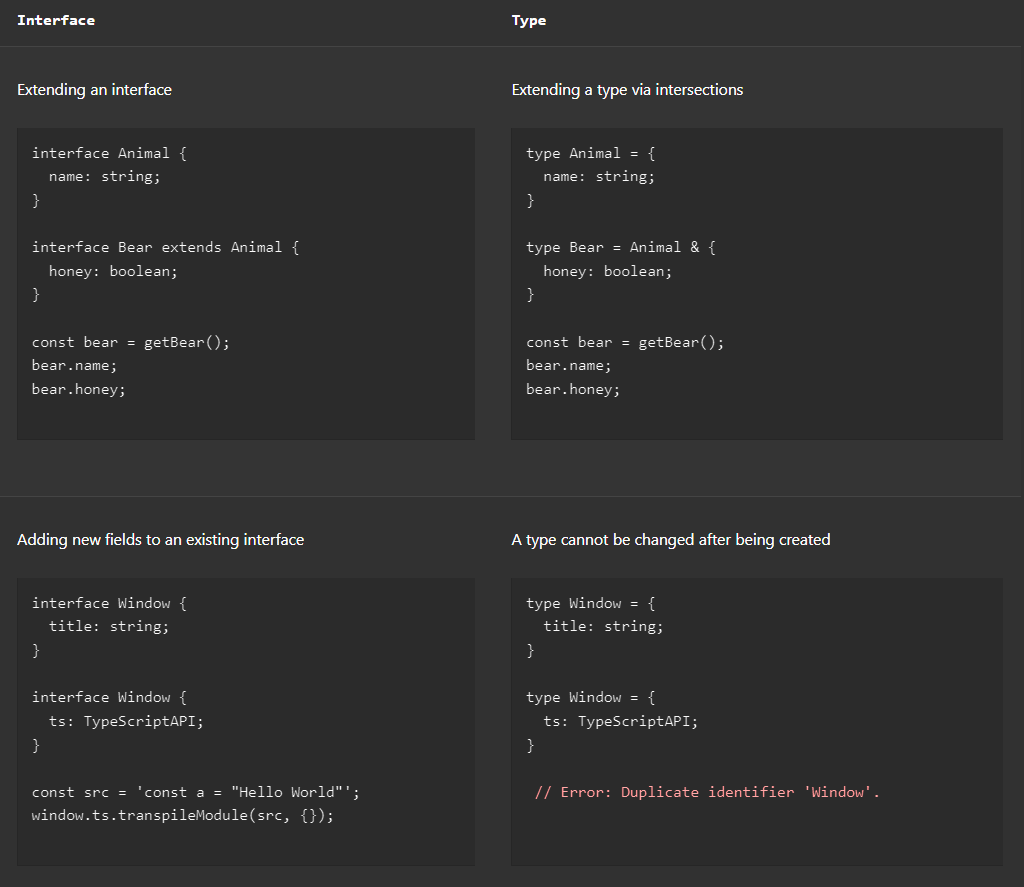
\includegraphics[width=\textwidth]{ss/4.png}
\end{figure}

Las interfaces no pueden crear tipos u objetos que estén altamente relacionados con los tipos primitivos (strings, numbers, bool, etc.), los types alias si pueden mediante las template union types, además de que estos alias pueden seleccionar entre varios tipos cuál resultarán siendo.

Para temas de clases, objetos y POO en general, podríamos seleccionar las interfaces, fuera de eso, nos podemos quedar con los alias sin ningún problema.



\section{Narrowing}

El concepto \textbf{narrowing} se refiere a que aseguremos que una constante o variable sea del tipo esperado para utilizar los métodos de su tipo, el narrowing podría verse como la solución a un problema que puede llegar a ocurrir con los unions types, tenemos el siguiente ejemplo:
\begin{lstlisting}
function mostrarLongitud(objeto: number | string) {
    return objeto.length // da error.
}
\end{lstlisting}

Si utilizamos el ejemplo anterior así como viene, al retornar la longitud del parámetro \textit{objeto} nos da un error porque este parámetro puede ser un número o una cadena, el método \textit{length} solo funciona con cadenas, para poder solucionar esto, podemos aplicar una condicional:
\begin{lstlisting}
function mostrarLongitud(objeto: number | string) {
    if(typeof objeto == 'string') {
        return objeto.length
    }

    return objeto.toString().length()
}
\end{lstlisting}

Esta solución es para tipos básicos, probemos ahora con una interface (se puede sustituir por un tipo más robusto):
\begin{lstlisting}
interface Mario {
    company: 'nintendo',
    name: string,
    saltar: () => void
}

interface Sonic {
    company: 'sega',
    name: string,
    correr: () => void
}

type Personaje = Mario | Sonic

function jugar(personaje: Personaje) {
    console.log(personaje.correr()) // da error.
}
\end{lstlisting}

Con estas estructuras más robustas resolveremos el problema de los tipos asignado a otro tipo. Se tienen dos interfaces y a un tipo nuevo se le asigna una de las interfaces o la otra, ambas comparten atributos (\textit{company} y \textit{name}) pero su atributo característico es el de \textit{saltar} o \textit{correr}, la función \textit{jugar} recibe un parámetro tipo Personaje y es aquí donde el problema comienza, TS no puede saber qué método va a llegar, por lo que nos da un error, para solucionarlo se hace una comprobación antes de mandarlo a llamar:
\begin{lstlisting}
interface Mario {
    company: 'nintendo',
    name: string,
    saltar: () => void
}

interface Sonic {
    company: 'sega',
    name: string,
    correr: () => void
}

type Personaje = Mario | Sonic

function jugar(personaje: Personaje) {
    if(personaje.company == 'nintendo') {
        personaje.saltar()
        return
    }
    
    personaje.correr()
}
\end{lstlisting}

Problema resuelto.


\subsection{Type guard}

Si queremos resolverlo sin la existencia de este atributo \textit{company} hay otro método, que es mediante una función bajo la técnica \textbf{type guard}: esta técnica nos pide realizar una función para asegurar que un parámetro es de un tipo en específico según un atributo de este tipo que lo diferencie de otros similares, la sintaxis de esta técnica para este ejemplo es la siguiente:
\begin{lstlisting}
function checkIsSonic(personaje: Personaje): personaje is Sonic {
    return (presonaje as Sonic).correr != undefined
}
\end{lstlisting}

Este método por defecto toma el parámetro recibido como un objeto tipo Sonic, si el resultado del método \textit{correr} del parámetro es \textit{undefined}, entonces el parámetro no es del tipo Sonic, de esta manera no necesitamos poner alguna condicional en nuestro código principal.

El narrowing y el type guard utilizan otro concepto normalmente llamado \textbf{discriminación de tipos}, el cual consiste en tomar tomar preferencia de un tipo sobre otro con baso a un atributo diferenciador, como podemos ver, estas técnicas siguen ese concepto para validación de datos y tipos. El código completo de este ejemplo con type guard es:
\begin{lstlisting}
interface Mario {
    company: 'nintendo',
    name: string,
    saltar: () => void
}

interface Sonic {
    company: 'sega',
    name: string,
    correr: () => void
}

type Personaje = Mario | Sonic

function checkIsSonic(personaje: Personaje): personaje is Sonic {
    return (presonaje as Sonic).correr != undefined
}

function jugar(personaje: Personaje) {
    if(checkIsSonic(personaje)) {
        personaje.correr()
        return
    }
    
    personaje.saltar()
}
\end{lstlisting}

\textit{Nota}: SE RECOMIENDA NO UTILIZAR TAN SEGUIDO EL TYPE GUARD, ya que conlleva realizar más comprobaciones y código.



\section{Encapsulamiento de atributos de Clases}

JS puede manejar la creación de clases al igual que el encapsulamiento de sus atributos según el enfoque esperado (privado o público), se puede agregar un \# al inicio de un atributo para indicar que este es privado, al mismo tiempo que hay una convención que es agregar un \_ al inicio de un atributo para indicar que este no debe ser modificado ni accedido directamente, pero igual podemos trabajarlo como un atributo público. TS si agrega los modificadores de acceso para lograr el encapsulamiento exitosamente, estos modificadores son \textbf{private}, \textbf{public} y \textbf{protected}, si tienes conocimiento sobre POO sabrás para que sirven y cual es el predefinido si no se define un modificador a un atributo o método.
\begin{lstlisting}
class Avenger {
    private name: string
    private powerScore: number
    private wonBattles: number

    constructor(name: string, powerScore: number) {
        this.name = name
        this.powerScore = powerScore
    }

    get fullName() {
        return `${this.name}, de poder ${this.powerScore}`
    }
    set power(newPower: number) {
        if(newPower <= 100) {
            this.powerScore = newPower
        }
        else {
            throw new Error('Power score cannot be more than 100')
        }
    }
}

const avenger = new Avenger('spidey', 80)
avenger.name = 'Hulk' // da error.
console.log(avenger.fullName()) // no da error.
\end{lstlisting}

Cuando decimos que podemos agregar un \# o \_ al inicio del nombre de un atributo o método en JS es porque de esta manera lo volvemos privado o aplicamos una convención para tratarlo como miembro privado, TS es el que tiene explícitamente un modificador que vuelve un miembro privado SOLO EN LA COMPILACIÓN, de preferencia utilizar lo sugerido en JS para asegurar el alcance de los miembros en tiempo de ejecución. Aquí está el mismo código anterior pero con lo mencionado anteriormente:
\begin{lstlisting}
class Avenger {
    #name: string
    #powerScore: number
    #wonBattles: number

    constructor(name: string, powerScore: number) {
        this.#name = name
        this.#powerScore = powerScore
    }

    get fullName() {
        return `${this.#name}, de poder ${this.#powerScore}`
    }
    set power(newPower: number) {
        if(newPower <= 100) {
            this.#powerScore = newPower
        }
        else {
            throw new Error('Power score cannot be more than 100')
        }
    }
}
\end{lstlisting}



\section{Usando interfaces con clases}

Al igual que en otros lenguajes de programación para POO, podemos hacer que una clase implemente una clase:
\begin{lstlisting}
interface IAvenger {
    name: string
    powerScore: number
    wonBattles: number
}

class Avenger implements IAvenger {
    name: string
    powerScore: number
    wonBattles: number
    
    constructor(name: string, powerScore: number,
        wonBattles: number) {
        this.name = name
        this.powerScore = powerScore
        this.wonBattles = wonBattles
    }

    get fullName() {
        return `${this.name}, de poder ${this.powerScore}`
    }
    set power(newPower: number) {
        if(newPower <= 100) {
            this.powerScore = newPower
        }
        else {
            throw new Error('Power score cannot be more than 100')
        }
    }
}
\end{lstlisting}



\section{Convención \textit{types.d.ts}}

Una convención es una forma estándar de llevar a cabo una tarea u organizar la arquitectura de un proyecto. Una convención vista en el vídeo es que metan toda las declaraciones de interfaces en un solo archivo llamado \textbf{types.d.ts}, dentro de este archivo no se puede meter otro código que no sea la declaración de una clase.

Utilizando esta convención en el ejemplo anterior quedaría de la siguiente manera:

\textbf{types.d.js}
\begin{lstlisting}
// opcion 1.
export interface Avenger {
    name: string
    powerScore: number
    wonBattles: number
}

// opcion 2.
interface Avenger {
    name: string
    powerScore: number
    wonBattles: number
}

export default Avenger
\end{lstlisting}

\textbf{main.ts}
\begin{lstlisting}
import {type Avenger} from './types.d'

class Avenger implements IAvenger {
    name: string
    powerScore: number
    wonBattles: number
    
    constructor(name: string, powerScore: number,
        wonBattles: number) {
        this.name = name
        this.powerScore = powerScore
        this.wonBattles = wonBattles
    }

    get fullName() {
        return `${this.name}, de poder ${this.powerScore}`
    }
    set power(newPower: number) {
        if(newPower <= 100) {
            this.powerScore = newPower
        }
        else {
            throw new Error('Power score cannot be more than 100')
        }
    }
}
\end{lstlisting}


% Fin del documento.
\end{document}